\begin{pastexam}[label={px:df3-106-ds-03}]{地方三等資訊處理 106 年 第三題}
（申論；30 分）

給定如下圖所示之兩個環狀單向鏈結串列（circular singly linked list），並以 A，B 分別指向其中兩個串列中
的一個節點，另有一個指標 C 可以使用。請用類 C 之虛擬語言（C-like pseudo code）完成下列動作。
\begin{center}
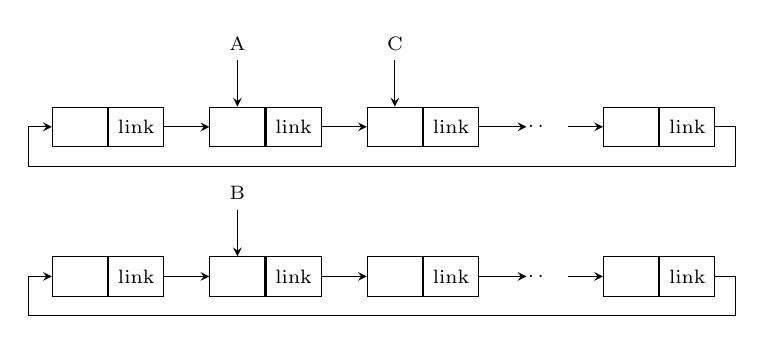
\begin{tikzpicture}[x=1cm, y=1cm, >=stealth, font=\scriptsize,
    nd/.style={draw, minimum height=5mm, minimum width=7mm, inner sep=0pt}]
\foreach \yy/\nm in {0/A, -1.9/B}{
  \foreach \k/\xx in {1/0, 2/2, 3/4, 4/7}{
    \node[nd] (\nm d\k) at (\xx,\yy) {};
    \node[nd, anchor=west] (\nm l\k) at (\nm d\k.east) {link};
  }
  \draw[->] (\nm l1.east) -- (\nm d2.west);
  \draw[->] (\nm l2.east) -- (\nm d3.west);
  \draw[->] (\nm l3.east) -- ++(0.6,0);
  \node at (5.75,\yy) {\dots};
  \draw[->] (6.2,\yy) -- (\nm d4.west);
  \draw[->] (\nm l4.east) -- ++(0.25,0) -- ++(0,-0.5) -- ([xshift=-0.3cm, yshift=-0.5cm]\nm d1.west) |- (\nm d1.west);
}
\draw[->] (2,0.85) node[above] {A} -- (Ad2.north);
\draw[->] (4,0.85) node[above] {C} -- (Ad3.north);
\draw[->] (2,-1.05) node[above] {B} -- (Bd2.north);
\end{tikzpicture}
\end{center}
\begin{enumerate}[leftmargin=2.2em]
\item[㈠] 請用至多二行虛擬碼程式刪除 C 所指向節點。結果必須維持環狀單向鏈結串列。（5 分）
\item[㈡] 請用至多二行虛擬碼程式將 B 所指向串列插入 A 所指向串列。結果必須維持環狀單向鏈結串列。（10 分）
\item[㈢] 請用至多四行虛擬碼程式寫出可將 B 所指向節點插入至 A 所指向節點之「前」，但必須維持環狀單向
鏈結串列。（15 分）
\end{enumerate}
\end{pastexam}

\begin{pastsoln}
節點有資料欄和 \texttt{link} 欄。 從圖上看，C 指向的節點就是 A 的下一個節點（\texttt{C == A->link}）。
三小題各自獨立，都從圖上的狀態開始。 單向串列只能往後走，所以操作的關鍵都是「改前一個節點的
\texttt{link}」（資結書第~5.2~節）。

\textbf{㈠ 刪除 C 所指的節點。}
\begin{minted}[fontsize=\small]{c}
A->link = C->link;
free(C);
\end{minted}
A 正好是 C 的前一個節點，讓 A 直接跳過 C 接到 C 的下一個節點，環就少了 C，仍然是一個環。 然後
把 C 的記憶體還回去。 （若 A、C 是同一個節點，也就是串列只剩一個節點，刪掉後串列變空，要另外把
A 設成 \texttt{NULL}；圖上至少有四個節點，不會發生。）

\textbf{㈡ 把 B 所在的串列併進 A 所在的串列。}
\begin{minted}[fontsize=\small]{c}
C = A->link;  A->link = B->link;
B->link = C;
\end{minted}
做法是把兩個環各在一處剪開，交叉接起來。 設 A 的下一個是 $a'$、B 的下一個是 $b'$：
\begin{itemize}
\item 原本：A → $a'$ → \dots → A，B → $b'$ → \dots → B。
\item 之後：A → $b'$ → \dots（B 的串列）\dots → B → $a'$ → \dots（A 的串列）\dots → A。
\end{itemize}
從 A 出發沿 \texttt{link} 走，會先走完 B 原本的整個環、回到 B，再接回 A 原本的環，最後回到 A，
所有節點串成一個環。 這就是交換 \texttt{A->link} 和 \texttt{B->link}，C 當暫存。 任一串列只有一個
節點時（例如 \texttt{B->link == B}）也對：得到 A → B → $a'$ → \dots → A。 時間 $O(1)$。

\textbf{㈢ 把 B 所指的節點插到 A 所指節點的前面。} 這裡把 B 當成一個要插入的單獨節點（它原本串列
的其他節點不管）。 插在 A 前面要改 A 的前一個節點的 \texttt{link}，單向環狀串列只能從 A 繞一圈找到它：
\begin{minted}[fontsize=\small]{c}
C = A;
while (C->link != A) C = C->link;
C->link = B;
B->link = A;
\end{minted}
第 1、2 行讓 C 從 A 往後走，停在 \texttt{link} 指向 A 的那個節點，也就是 A 的前一個節點；第 3、4 行把
B 接在 C 和 A 中間：C → B → A。 環的其他部分沒動，仍然是環狀串列。 只有一個節點（\texttt{A->link == A}）
時迴圈不執行，C 就是 A，結果是 A → B → A，也對。 時間 $O(n)$，$n$ 是 A 所在串列的節點數。

另一種 $O(1)$ 的做法是「插在後面再交換資料」：先 \texttt{B->link = A->link; A->link = B;} 把 B 接在 A
後面，再交換 A、B 兩個節點的資料欄。 這樣資料的順序是「B 的資料、A 的資料」，看起來 B 在 A 前面，
但 A 這個指標現在指的節點裝的是 B 的資料，若之後還要用 A 指原本那筆資料，要再加一行 \texttt{A = B;}，
總共超過四行，而且節點的資料很大時交換也不便宜。 題目限四行，用上面找前驅的寫法最直接。
\end{pastsoln}
